\section{Big data arhitektura}

\subsection{Arhitektura aplikacij}
Aplikacijska arhitektura opisuje načine in tehnike, ki so uporabljene pri zasnovi in gradnji aplikacije.
Arhitektura nam olajša načrtovanje poteka razvoja in nam poda dobre prakse za grajenje aplikacij~\cite{application_architecture_def}.
Skozi čas se je razvilo več tipov arhitektur, spodaj opišemo samo nekatere.

\paragraph{Monolitna arhitektura}
Vse funkcionalnosti so združene skupaj v eni aplikaciji.
Za vsako posodobitev moramo ponovno izdati celo aplikacijo in različne funkcionalnosti so močno povezane.

\paragraph{Mikrostoritve}
Aplikacije razbijemo na najmanjše dele, ki so neodvisni en od drugega.
Vsako mikrostoritev lahko posodobimo neodvisno, funkcionalnosti so neodvisne ena od druge.

\paragraph{Arhitektura vodena preko dogodkov}
Imamo proizvajalce in porabnike dogodkov.
Proizvajalci se ne zavedajo porabnikov, kar pomeni večjo neodvisnost.
Z dodajanjem novih proizvajalcev in porabnikov lahko arhitekturo enostavno skaliramo.

\subsection{Izzivi big data arhitekture}
\todo{Primerjava s tradicionalno arhitekturo}
Avtorji v članku~\cite{provisioning_big_data_micro_cloud} predstavijo težave dinamičnega priskrbovanja big data aplikacij.
Predstavijo naslednje izzive.

\paragraph{Konfiguracija in postavljanje}
Tehnologije, ki so uporabljene v arhitekturi so ponavadi kompleksne in imajo veliko parametrov.
Za njihovo nastavitev potrebujemo zaposlene z znanjem teh tehnologij in že majhna napaka lahko pomeni slabše
delovanje.

\paragraph{Elastičnost}
Obremenitve aplikacije se lahko hitro spreminjajo.
Želimo jih hitro zaznati in se jim prilagoditi, saj s tem prihranimo denar, ali pa preprečimo počasno delovanje
ob nenadnih poskokih zahtevnosti.

\paragraph{Visoka razpoložljivost}\label{par:high_availability}
Napake so v aplikacijah pričakovane, saj lahko pride do napak v strojni opremi, napak v samih aplikacijah ali
napak pri komunikaciji med aplikacijami.
Napakam se moramo znati prilagoditi in zmanjšati čas, ko je naša aplikacija nedosegljiva.
Preprečiti moramo izgube ali nedosegljivosti podatkov.
Članek~\cite{ha_computer_systems} opiše visoko dosegljivost in načine, kako jo lahko dosežemo.
Grobo, visoka dosegljivost pomeni, da mora biti naša aplikacija dostopna 99.999\% časa, kar pomeni, da je lahko
nedostopna 5 minut na leto.

\paragraph{Sobivanje aplikacij}
\todo{Dodaj prevode: multy-tenancy}
Aplikacije različnih strank kdaj bivajo v istem okolju.
Aplikacije morajo biti med sabo izolirane in aplikacija ene stranke ne sme povzročiti izpada aplikacije 
neke druge stranke.

\paragraph{Verzioniranje in podpiranje različnih verzij}
Želimo imeti vodenje verzij aplikacije in različnih tehnologij, ki so uporabljene za podporo aplikacije.
V nekaterih primerih moramo hkrati ponujati več različnih verzij iste aplikacije 
ali njihovih podpornih komponent saj ni nujno, da vsi odjemalski sistemi podpirajo 
ali so prilagojeni za delovanje na najnovejših verzijah podpornih tehnologijah.

\paragraph{Ostali izzivi}
Varnost in upoštevanje licenc, ki pa nista značilni samo za big data aplikacije.

\subsection{Arhitekturi Kappa in Lambda}

Arhitekture Big Data so raznolike,
ampak okvirno jih lahko uvrstimo v dva razreda: Kappa ali Lambda arhitekturo~\cite{kappa_lambda}.
Lambda arhitektura vsebuje storitve za procesiranje podatkovnih tokov
in za procesiranje paketov, medtem ko Kappa vsebuje samo storitve za
procesiranje tokov in delo s paketi obravnava kot tokove z zakasnitvijo.

Kappa in Lambda predstavljata dva načina razmišljanja in sicer posploševanje in
specializacija.
Kappa je posplošena, kar pomeni da nam ni treba pisati konfiguracij
za storitve za delo s paketi in ni usklajevanja med storitvami,
ampak zaradi tega je delovanje počasnejše, kot če bi imeli orodje,
ki je specializirano za delo s paketi.
Pri Lambdi je problem ravno obraten, imamo pravo orodje,
ampak moramo usklajevati konfiguracijo med storitvami za tokove in za pakete.

\subsection{Primeri big data arhitektur}

V tem odseku predstavimo nekaj arhitektur znanih podjetij~\cite{reference_architecture_classification_technologies}.
Na koncu predstavimo referenčno arhitekturo,
ki je povzeta iz članka~\cite{reference_architecture_classification_technologies} in je
podobna referenčni arhiteturi iz članka~\cite{reference_architecture_bd}.
Arhitektura Facebooka je predstavljena v sliki~\ref{fig:arch-facebook}, arhitektura Twitterja pa v sliki~\ref{fig:arch-twitter}.

\begin{figure}[H]
    \centering
    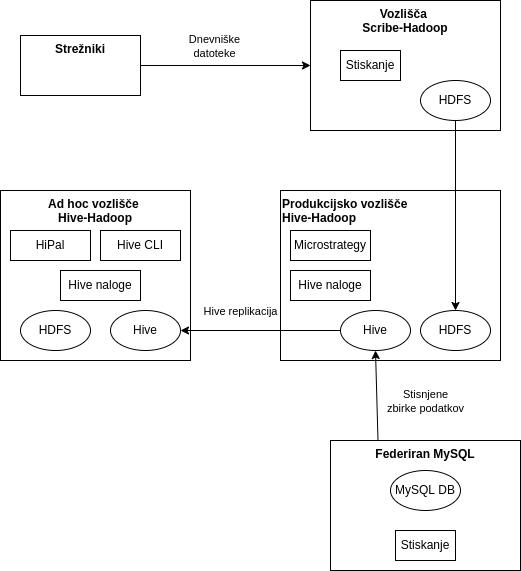
\includegraphics[width=0.6\textwidth]{img/arhitektura/podjetja/facebook.png}
    \caption{Arhitektura za analizo podatkov pri Facebook~\cite{reference_architecture_classification_technologies}.}
    \label{fig:arch-facebook}
\end{figure}

\begin{figure}[H]
    \centering
    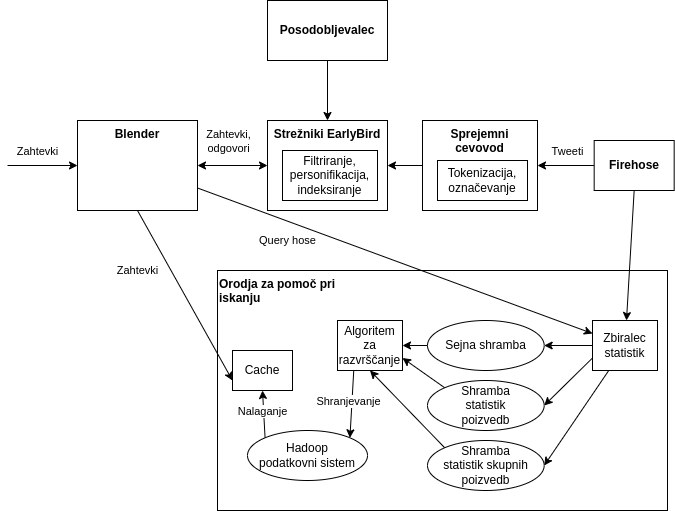
\includegraphics[width=0.8\textwidth]{img/arhitektura/podjetja/twitter.png}
    \caption{Arhitektura za analizo podatkov pri Twitterju~\cite{reference_architecture_classification_technologies}.}
    \label{fig:arch-twitter}
\end{figure}

\noindent Iz več primerov arhitektur, avtorji članka~\cite{reference_architecture_classification_technologies}
ustvarijo referenčno arhitekturo za Big Data, ki je predstavljena v sliki~\ref{fig:arch-ref-article}.

\begin{figure}[H]
    \centering
    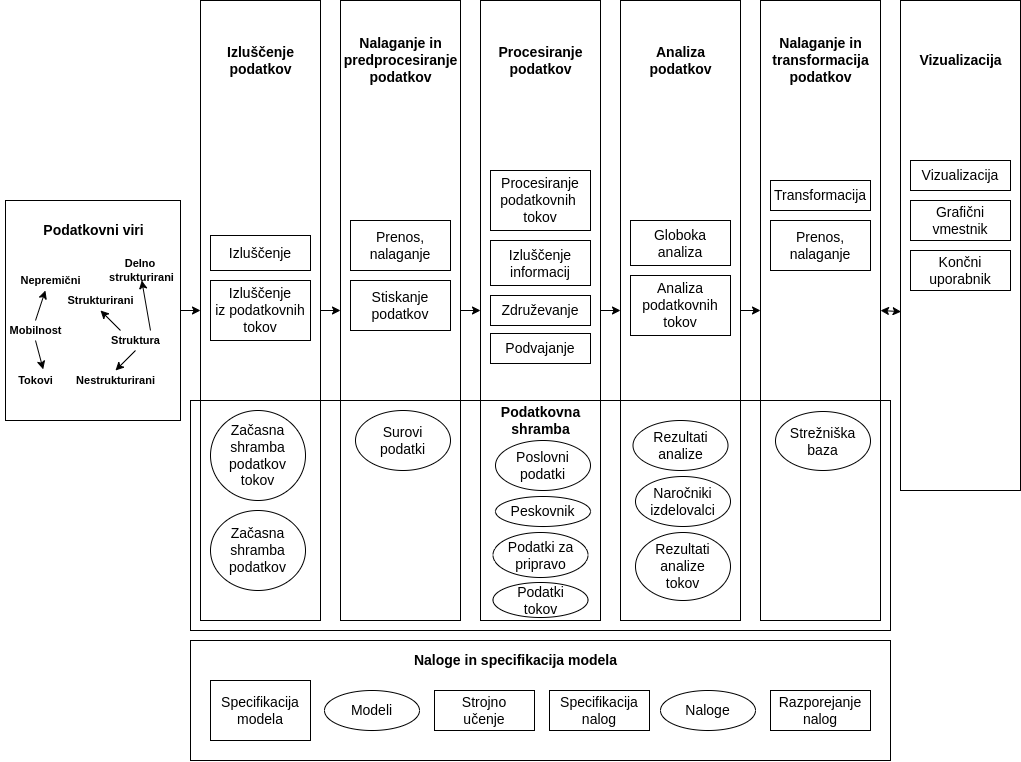
\includegraphics[width=0.99\textwidth]{img/arhitektura/reference.png}
    \caption{Visoko nivojska referenčna arhitektura Big Data aplikacij.
        Podatkovne shrambe so prikazane v elipsah, storitve v kvadratih in
        pot podatkov s puščicami.
        Povzeto po članku~\cite{reference_architecture_classification_technologies}.}
    \label{fig:arch-ref-article}
\end{figure}

\noindent V poglavju~\ref{sec:metodologija} referenčno arhitekturo uporabimo skupaj z
iteracijsko metodo~\cite{iterative_methodology} in
naredimo metodologijo.

\paragraph{Shramba}
Relacijske baze niso primerne za uporabo z nestrukturiranimi podatki.
Prav tako so te baze počasnejše kot NoSQL podatkovne baze,
kar nas omejuje pri analizi big data, saj je hitrost ključnega pomena.
NoSQL podatkovne baze sprostijo strukturo, kar olajša delo z nestrukturiranimi podatki.
Prav tako NoSQL baze omilijo zahteve glede konsistence in
omogočajo večjo dosegljivost in večjo skalabilnost.

V naši metodologiji bomo uporabili Opensearch~\cite{tech_opensearch}, 
ki je odprtokodna veja podatkovne baze Elasticsearch.
Opensearch je NoSQL podatkovna baza, ki omogoča visoko skalabilnost.

\paragraph{Procesiranje podatkov}
Pri delu z big data bomo delali s podatkovnimi tokovi
in potrebujemo orodje, ki je neodvisno od tipa podatkov in omogoča delo z veliko količino podatkov.
Želimo imeti visoko dostopnost in orodje mora ohranjati kvaliteto podatkov.

Uporabili bomo Apache Kafka~\cite{tech_kafka}.
Članek~\cite{iterative_methodology} opisuje Kafkine lastnosti.
Kafka omogoča obdelavo visoke količine podatkov v realnem času.
Podatki so lahko raznoliki in podpira uporabo strukturiranih in nestrukturiranih podatkov.
Kafko garantira, da se podatki ne izgubijo in ne podvojijo.